% Current evaluation chapter, authored 06/10/2026. Earlier development chapters
% and sealed evidence are retained. Compile from thesis/ as part of main.tex.
\chapter{Đánh giá thực nghiệm và phạm vi kết luận}
\label{ch:experiments}
% Generated by experiments/export_thesis_evaluation_20261006.py; do not hand-edit.
\newcommand{\EvalFreshPurposeRows}{%
Gần nhất & 92,449 & 94,680 & +2,230 & [1,741; 2,732] \\
Nhanh nhất & 92,449 & 94,678 & +2,229 & [1,741; 2,731] \\
Trong bán kính & 81,694 & 86,879 & +5,185 & [3,992; 6,396] \\
Ít vòng đường nhất & 92,266 & 94,516 & +2,250 & [1,733; 2,798] \\
Trung bình đều purpose & 89,714 & 92,688 & +2,974 & [2,308; 3,646] \\
}

% Generated by experiments/export_thesis_evaluation_20261006.py; do not hand-edit.
\newcommand{\EvalFreshCostRows}{%
L20 & 90\,570 & 13\,678\,985 & 494\,713\,236 \\
L30 & 90\,570 & 13\,678\,985 & 648\,578\,577 \\
}

% Generated by experiments/export_thesis_evaluation_20261006.py; do not hand-edit.
\newcommand{\EvalMatchedAnchorRows}{%
GPS thật & 100,0 & 100,0 & 100,000 & 100,000 \\
REM--Geo-I & 50,0 & 50,0 & 94,693 & 99,905 \\
Planar--Geo-I & 50,0 & 50,0 & 96,999 & 99,352 \\
}

% Generated by experiments/export_thesis_evaluation_20261006.py; do not hand-edit.
\newcommand{\EvalEndpointRows}{%
GPS thật & 100,00 / 0,0 / 100,00 & 100,00 / 0,0 / 100,00 \\
GeoI-Slack L20 & 1,79 / 789,9 / 24,11 & 0,00 / 757,7 / 12,50 \\
GeoI-Endpoint20 & 0,00 / 1406,7 / 7,14 & 0,00 / 1337,2 / 4,46 \\
}

% Generated by experiments/export_thesis_evaluation_20261006.py; do not hand-edit.
\newcommand{\EvalHistoricalLocationRows}{%
GPS thật & 100,00 / 13 / 100,00 & 100,00 / 39 / 100,00 & 96,43 / 23 / 100,00 \\
DLS* & 58,33 / 1318 / 100,00 & 100,00 / 39 / 100,00 & 31,21 / 1688 / 100,00 \\
TransProtect* & 83,33 / 84 / 97,78 & 66,67 / 88 / 97,19 & 69,28 / 99 / 97,93 \\
Semantic* & 100,00 / 11 / 100,00 & 100,00 / 42 / 100,00 & 40,58 / 257 / 100,00 \\
BR--Geo-I lịch sử & 33,33 / 299 / 95,83 & 22,22 / 247 / 97,01 & 7,44 / 776 / 87,67 \\
}

% Generated by experiments/export_thesis_evaluation_20261006.py; do not hand-edit.
\newcommand{\EvalRejectedPlannerRows}{%
Vòng 1 & \texttt{aligned\_nearest} & -0,061 & Thiếu gain \\
Vòng 1 & \texttt{multi\_mean} & -0,411 & Thiếu gain \\
Vòng 1 & \texttt{tail25} & 0,437 & Thiếu gain; không qua S5/S6 \\
Vòng 1 & \texttt{tail50} & 0,433 & Thiếu gain; không qua S5/S6 \\
Vòng 2 & \texttt{aligned\_nearest} & -0,061 & Thiếu gain \\
Vòng 2 & \texttt{normalized\_mean} & 0,118 & Thiếu gain \\
Vòng 2 & \texttt{normalized\_tight} & -0,345 & Thiếu gain \\
Vòng 2 & \texttt{normalized\_tail} & -0,344 & Thiếu gain \\
}


Kết quả hiện tại cho thấy hệ thống có thể giữ nền tảng Geo-I, phục vụ nhiều mục
đích tìm POI tại thiết bị và cải thiện chất lượng trả lời bằng một thay đổi công
khai ở phía dịch vụ. Trên tập xác nhận mới cùng bản đồ, tăng độ sâu phản hồi từ
L20 lên L30 làm Recall@5 trung bình tăng \EvalFreshGain{} điểm phần trăm, với
khoảng tin cậy ghép theo nhóm tuyến là
[\EvalFreshLow{}; \EvalFreshHigh{}] điểm phần trăm. Đổi lại, byte phản hồi tăng
\EvalReplyGrowth{}\%. Cùng những tọa độ Q, lịch gửi, neo và sổ ngân sách được
giữ nguyên. Đây là kết quả điều chỉnh utility--cost của dịch vụ tĩnh, không phải
một thuật toán Geo-I mới hoặc một chứng minh thắng các đối chứng ở cùng chi phí.

Các phép thử suy luận tương lai, liên kết phiên và điểm đầu/cuối bổ sung bằng
chứng cho luận văn, nhưng có phạm vi khác nhau. Vì vậy chương này trình bày
riêng kết quả xác nhận mới, các chẩn đoán phát triển đã được xem và những tác vụ
chưa đo. Không ghép chúng thành một bảng xếp hạng riêng tư duy nhất.

\section{Thiết kế đánh giá và mức độ bằng chứng}
\label{sec:current-evidence-design}

\subsection{Tách dữ liệu phát triển khỏi xác nhận mới}

Mỗi thí nghiệm có protocol, dữ liệu, đầu ra công khai, nhãn chỉ dành cho bộ
đánh giá, nguồn mã đã đóng băng và bản kiểm chứng riêng. Một kết quả kiểm chứng
PASS xác nhận các điều kiện mà checker thực sự kiểm tra, chẳng hạn hash nguồn,
ngân sách đã chi, mẫu số và phép tính metric. Nó không tự chứng nhận theorem
Geo-I, độ mạnh tối ưu của attacker hoặc hiệu quả trong triển khai thực tế.

Ba nhóm bằng chứng được sử dụng như sau.
\begin{enumerate}
  \item \textbf{Phát triển lịch sử.} Paper-v2 đo S1--S3 và S9--S10 trên các
  adaptation; những vòng endpoint, S4, S7 và planner tiếp theo đã sử dụng lại
  hoặc đã đọc các nhóm đánh giá. Chúng là chẩn đoán phát triển, kể cả khi tệp
  có tên \texttt{test}.
  \item \textbf{Pilot native có kiểm soát.} Mạng đường mới được biên dịch từ
  hình học lưu trữ và dùng nhất quán để sinh chuyển động SUMO, bảo vệ, truy hồi
  POI và giải mã cạnh. Các pilot có 24 nhóm tuyến, chia 12/6/6 nhóm
  train/selection/test. Kết quả này kiểm tra các quyết định và cơ chế cụ thể;
  những extension được thiết kế sau khi xem pilot vẫn là phát triển.
  \item \textbf{Xác nhận utility đã khóa.} Sau hai vòng planner không đạt gate,
  chỉ chính sách độ sâu công khai L30 được chọn và đóng băng trước khi sinh và
  chấm cohort mới. Cohort có 60 nhóm tuyến native, chia 24/12/24 nhóm; số lần
  ngẫu nhiên theo ba phần là 1/1/3. Phần test gồm 24 nhóm, mỗi nhóm ba lần
  ngẫu nhiên và tám phiên. Chỉ L20 và L30 được chấm ở bước xác nhận.
\end{enumerate}

Các mạng mới giữ đúng lane, turn và edge ID cho chính mạng SUMO được tạo.
Chúng không phải bản phục hồi đầy đủ mạng Beijing gốc. Toàn bộ dữ liệu vẫn là
mô phỏng trên một khu vực và một bộ POI công khai. Cohort mới giảm việc chọn
cấu hình theo đáp án đã xem, nhưng không thay thế xác nhận khác thành phố,
GPS thật hoặc dữ liệu dịch vụ thật.

\subsection{Trạng thái S1--S10}

Trong Bảng~\ref{tab:current-scenario-coverage}, ``thực nghiệm'' nghĩa tác vụ
đã có đầu vào và metric chạy được; không có nghĩa scenario đã được giải quyết
đầy đủ. ``Lý thuyết'' chỉ bảo đảm có điều kiện của kernel Geo-I và phép hợp
thành. ``Proxy'' là một đại diện hẹp hơn target đã định nghĩa.

\begingroup
\small
\setlength{\tabcolsep}{4pt}
\begin{longtable}{P{0.7cm}P{3.4cm}P{3.0cm}P{7.3cm}}
\caption{Phân loại bằng chứng hiện tại theo scenario.}\label{tab:current-scenario-coverage}\\
\toprule S & Target & Bằng chứng & Giới hạn khi kết luận \\\midrule
\endfirsthead
\toprule S & Target & Bằng chứng & Giới hạn khi kết luận \\\midrule
\endhead
S1 & Vị trí hiện tại & Thực nghiệm phát triển; lý thuyết tọa độ có điều kiện &
Paper-v2 có Hit100/MAE. Chưa có xác nhận S1 mới cho cấu hình L30; $\varepsilon$ không tự quyết định attack score. \\
S2 & Nơi dừng & Thực nghiệm phát triển &
Đo trên đoạn dừng có kiểm soát; chưa bao phủ mọi thời lượng, mức nhiễu GPS và thông tin phụ trợ về điểm dừng. \\
S3 & Đường đã đi & Thực nghiệm phát triển &
Giải mã chuỗi bằng bank hữu hạn. Validity/độ hợp lý của Q không phải metric riêng tư. \\
S4 & Cùng người hoặc phương tiện & Thực nghiệm nhãn tổng hợp; chưa đo metadata &
Tách người và xe; các cặp trong cùng family phụ thuộc. Không bảo vệ account, IP, biển số hay phần cứng bằng Geo-I. \\
S5 & Cạnh đường kế tiếp & Proxy cũ; thực nghiệm native ứng viên &
Pilot mới chấm edge thật tại fork hai lựa chọn; không phải dự báo cạnh trong thế giới mở. \\
S6 & Đích tương lai & Proxy cũ; thực nghiệm native có lịch sử &
Sáu lịch sử và prefix chuyến hiện tại, hai đích công khai. Chưa xét attacker đã liên kết tất cả chuyến truy vấn. \\
S7 & Nội dung hoặc ý định query & Kiểm thử bất biến request; thực nghiệm phát triển &
Đổi purpose local không đổi request có cùng protected state. Tương quan intent--location vẫn có thể tiết lộ ý định; không phải privacy vô điều kiện cho intent. \\
S8 & Suy luận từ người đồng hành & Chẩn đoán lịch sử, bank hữu hạn &
So bật/tắt quan sát đồng hành trên ba family. RNG lịch sử có seed tái tạo; chưa xác nhận cho Epoch8/L30, attacker biết seed hoặc privacy cấp nhóm. \\
S9 & Điểm xuất phát & Thực nghiệm endpoint phát triển &
Bank hình học và học có điều chỉnh theo output; cohort đã xem. Không đồng nhất che đầu, thêm nhiễu và ẩn thời điểm bắt đầu. \\
S10 & Điểm kết thúc & Thực nghiệm endpoint phát triển &
Giữ cả bank/selector thất bại. Hit100 bằng 0 ở hai phương pháp không chứng minh chênh lệch; chưa xác nhận endpoint trên cohort độc lập mới. \\
\bottomrule
\end{longtable}
\endgroup

\section{Metric chung và metric của công trình gốc}
\label{sec:current-metric-fairness}

Output của đối chứng không cùng loại: có phương pháp công bố một tọa độ thay
thế, có tập chứa tọa độ thật và dummy, có tập Q chỉ gồm tọa độ được bảo vệ,
hoặc một bộ quỹ đạo tổng hợp offline. Vì thế, một metric giả định có ``thành
viên thật trong tập công bố'' không thể được áp trực tiếp cho Q-only. Không
được gán ASR bằng 100\% chỉ vì tọa độ thật không có trong tập Q, hoặc biến một
failure của bộ sinh quỹ đạo thành thành tích riêng tư.

Đánh giá dùng hai lớp bổ sung. Lớp chung chấm target mà attacker suy ra từ
đúng output được cấp: MAE và Hit tại ngưỡng công khai cho vị trí; balanced
accuracy, log-loss hoặc AUC cho phân loại; Recall@5 cho POI; request/byte cho
chi phí. Lớp metric gốc chỉ tính khi có đủ input và đúng ý nghĩa của output.
Các ô thiếu dữ liệu giữ N/A cùng lý do.

\begin{table}[htbp]
\centering\small
\caption{Phạm vi metric gốc trong hồ sơ bằng chứng hiện tại.}
\label{tab:current-native-metrics}
\begin{tabularx}{\textwidth}{P{3.0cm}Y Y}
\toprule Metric & Có thể đọc từ evidence & Không được suy rộng \\\midrule
EIE dạng point estimate & Khi cùng decoder, khoảng cách và phép gộp, bằng MAE đã báo cáo. & Không phải một bằng chứng riêng tư độc lập thứ hai; posterior EIE cần posterior phù hợp. \\
$\Delta c$ của TransProtect & Một diagnostic riêng tính chi phí đường có hướng trên prior POI công khai. & Archive đối chứng thiếu cost table/prior gốc; diagnostic Q-only không lấp N/A hoặc chứng nhận tái lập paper. \\
Entropy, ASR, DER & Chỉ có nghĩa khi có prior/posterior, thành viên thật và quy tắc khả thi tương ứng. & Không áp trực tiếp cho Q-only; DER hay dummy hợp lý không đồng nghĩa attacker sai. \\
Số đường khó phân biệt & Cần quy tắc thời gian tới/hướng đi và số query kề nhau tương thích nguồn. & Không thay bằng số Q hoặc số đường hợp lệ trên bản đồ. \\
CoP/JSD/beacon linkage & Cần trạm sạc, dataset tổng hợp ghép cặp hoặc beacon/pseudonym trace đúng hợp đồng. & Không coi CoP, JSD, Recall và MAE là cùng một privacy score. \\
\bottomrule
\end{tabularx}
\end{table}

Một adaptation chưa đạt fidelity của mô hình học, output protocol và attacker
gốc được ghi dấu *. So sánh chung có ích để phản biện thiết kế, nhưng không
gọi là tái lập trung thành hoặc chứng minh thắng paper đã công bố. Ngoài split
và dữ liệu, cần đọc cùng số tọa độ gửi, chi phí phản hồi và tổng cap; hai
phương pháp có cùng metric không tự có cùng tài nguyên hoặc cùng bảo đảm.

\subsection{Mẫu số và khoảng tin cậy}

Với purpose $p$, category $c$ và thời điểm $t$, bộ tham chiếu $R_{p,c,t}$ được
xếp hạng từ GPS và điều kiện query riêng ở phía evaluator. Kết quả thiết bị
$A_{p,c,t}$ chỉ được lấy từ các POI đã nhận và còn hiệu lực. Khi tham chiếu
không rỗng,
\begin{equation}
 r_{p,c,t}=\frac{|A_{p,c,t}\cap R_{p,c,t}|}{|R_{p,c,t}|}.
 \label{eq:current-conditional-recall}
\end{equation}
Khi không có POI tham chiếu phù hợp hoặc tới được, metric là N/A. Không đổi
N/A thành 0 hoặc 1; đồng thời báo số category và cửa sổ có tham chiếu.

Kết quả fresh lấy trung bình category có tham chiếu tại mỗi event, rồi gộp các
event trong mỗi purpose, các lần ngẫu nhiên trong mỗi family và các purpose
được định nghĩa với trọng số đều. Cuối cùng mỗi family có cùng trọng số.
Các draw có cùng inventory tham chiếu. Số cửa sổ hoặc số request không được
dùng như số subject độc lập. Bootstrap ghép lấy lại toàn bộ family 10.000 lần
và giữ ba draw bên trong; báo percentile 2,5\% và 97,5\% của chênh lệch L30--L20.
Khoảng này mô tả biến thiên giữa nhóm tuyến của generator hiện tại, không
bao gồm bất định của thành phố khác, đo GPS thật hoặc lựa chọn thiết kế khác.

\section{Kết quả xác nhận: tăng độ sâu phản hồi trên cùng Q}
\label{sec:current-fresh-depth}

Hai vòng thử cải thiện mục tiêu chọn Q không đủ điều kiện được chọn. Bước
tiếp theo giữ planner \texttt{legacy\_l10}, chữ ký nội bộ L10, K=5 và top-5
local; chỉ tăng số POI tối đa cho mỗi category ở mỗi Q mà dịch vụ trả về.
L30 không có nghĩa 30 điểm nhiễu hay 30 lần đọc GPS. Các category được yêu cầu
và độ sâu là cấu hình công khai, không phụ thuộc purpose riêng.

Trên development, thử L20/30/40/60 và chọn độ sâu nhỏ nhất tăng utility ít nhất
2 điểm phần trăm, không giảm nearest và có byte phản hồi không quá 2,5 lần
L20. L30 được chọn dù L40/L60 cũng đủ gate; không chọn độ sâu theo điểm test.
Quy tắc fresh được khóa trước generation/scoring: mean gain ít nhất 2 điểm
phần trăm, cận dưới CI ghép 95\% dương và gain dương ở cả ba draw.

\begin{table}[htbp]
\centering\small
\caption{Fresh test: Recall@5 conditional theo purpose, phản hồi hiện tại, 24 family. Đơn vị Recall là \%; gain và CI là điểm phần trăm.}
\label{tab:current-fresh-purpose}
\begin{tabularx}{\textwidth}{Yrrrr}
\toprule Purpose & L20 & L30 & Gain & CI ghép 95\% \\\midrule
\EvalFreshPurposeRows
\bottomrule
\end{tabularx}
\end{table}

Cả ba điều kiện fresh đều đạt. Gain theo draw là
\EvalDrawOne{}, \EvalDrawTwo{} và \EvalDrawThree{} điểm phần trăm. Trung bình
của 25\% family có utility thấp nhất tăng từ \EvalTailLowBefore{}\% lên
\EvalTailLowAfter{}\%; đây là chênh lệch của hai tail mean, không phải tail
mean của các chênh lệch. Các khoảng theo purpose và tail là phân tích phụ,
chưa hiệu chỉnh nhiều phép so sánh.

Purpose within-radius có \EvalRadiusDefinedCategories{}/\EvalRadiusTotalCategories{}
category references và \EvalRadiusDefinedWindows{}/\EvalRadiusTotalWindows{}
cửa sổ được định nghĩa. Ba purpose còn lại có toàn bộ tham chiếu category
được định nghĩa trong test. Gain trong Bảng~\ref{tab:current-fresh-purpose}
vì vậy là chất lượng có điều kiện trên nơi có tham chiếu; tăng L không tạo ra
POI ở nơi không có mục tiêu phù hợp. GPS và điểm đến riêng của evaluator dùng
để chấm utility tại event không đi vào planner Q hay server.

\begin{table}[htbp]
\centering\small
\caption{Chi phí JSON ứng dụng trên fresh test. Mỗi bộ phản hồi tính cả POI trùng giữa các Q.}
\label{tab:current-fresh-cost}
\begin{tabular}{lrrr}
\toprule Cấu hình & Requests & Request bytes & Reply bytes \\\midrule
\EvalFreshCostRows
\bottomrule
\end{tabular}
\end{table}

Byte phản hồi tăng \EvalReplyGrowth{}\%, còn request và request bytes giữ
nguyên. Đây là lượng compact JSON được tính từ bản tin thực trong simulator;
chưa đo HTTP/TLS, latency, pin hoặc chi phí nhà cung cấp. Không diễn giải lịch
đọc GPS bảo vệ cách 60 giây thành mức tiết kiệm năng lượng điện thoại.

Kiểm chứng độc lập đã xác nhận nguyên vẹn 108 bundle, bản tin Q/lịch gửi,
neo và ledger; tái dựng utility/cost L20, prefix L30 và các phép tính ghép
family. Kết quả current-only là primary. Cache tĩnh theo epoch tăng từ
98,808\% lên 99,136\%, chỉ 0,328 điểm phần trăm, là kết quả phụ khác hợp đồng
current-only; không dùng số cache để thay điểm primary.

\begin{figure}[H]
\centering
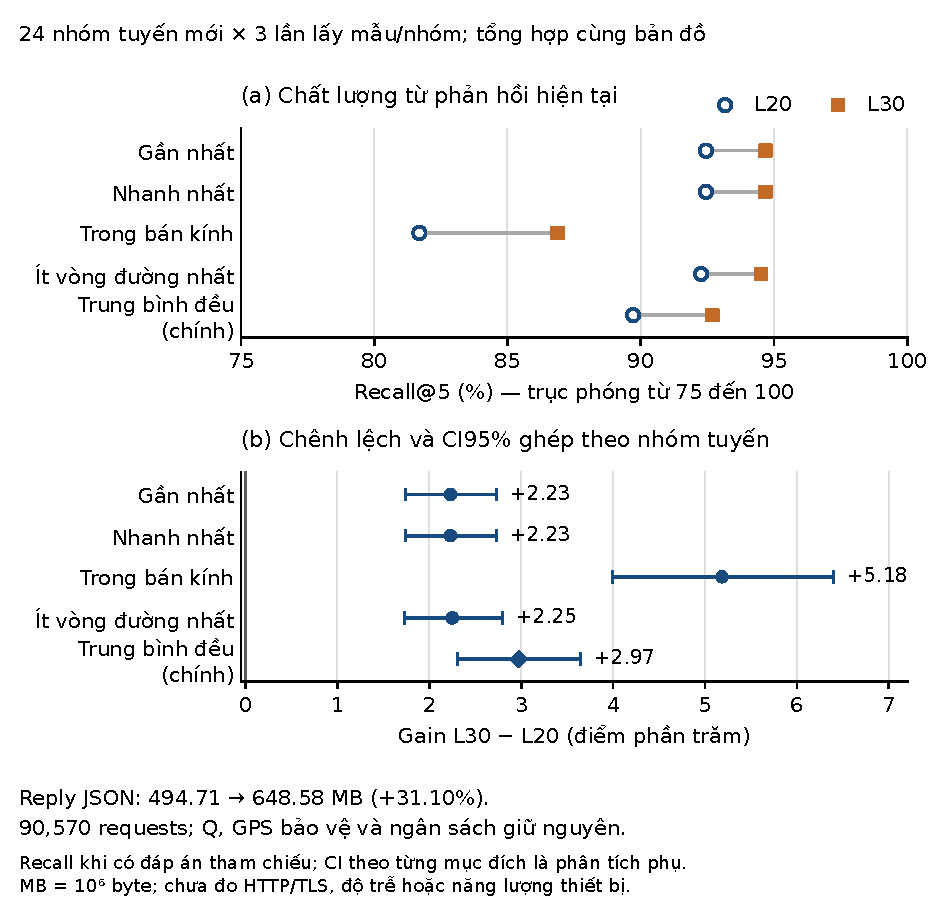
\includegraphics[width=\textwidth]{../artifacts/reports/thesis_figures_20261006/depth_utility_cost.pdf}
\caption{Fresh L30--L20: Recall có điều kiện và CI95\% ghép nhóm trên cùng Q. Trục Recall phóng từ 75--100\%; khoảng theo purpose là phân tích phụ chưa hiệu chỉnh nhiều phép so sánh. Hình định dạng lại thống kê đã lưu, không chấm thêm cấu hình trên fresh.}
\label{fig:current-depth-utility-cost}
\end{figure}

% Generated by experiments/export_thesis_extensions_20261007.py; do not hand-edit.
\newcommand{\SensorRowsSeven}{%
GPS chính xác mỗi event & 0,0 & 6,5 & 89,71 & 92,69 \\
Giữ fix, $\sigma=0$ m & 66,3 & 69,9 & 86,74 & 89,35 \\
Giữ fix, $\sigma=5$ m & 70,3 & 70,7 & 84,53 & 86,93 \\
Giữ fix, $\sigma=15$ m & 78,5 & 76,5 & 82,77 & 85,02 \\
Ngoại suy, $\sigma=0$ m & 56,8 & 59,4 & 85,78 & 88,28 \\
Ngoại suy, $\sigma=5$ m & 61,6 & 60,9 & 83,80 & 86,13 \\
Ngoại suy, $\sigma=15$ m & 72,5 & 68,8 & 82,54 & 84,77 \\
}
\newcommand{\SensorThreePurposeRows}{%
GPS chính xác mỗi event & 88,86 & 92,08 \\
Giữ fix, $\sigma=0$ m & 85,19 & 87,97 \\
Giữ fix, $\sigma=5$ m & 82,51 & 85,05 \\
Giữ fix, $\sigma=15$ m & 80,44 & 82,81 \\
Ngoại suy, $\sigma=0$ m & 84,07 & 86,73 \\
Ngoại suy, $\sigma=5$ m & 81,68 & 84,14 \\
Ngoại suy, $\sigma=15$ m & 80,18 & 82,54 \\
}
\newcommand{\SensorSafetyRows}{%
GPS chính xác mỗi event & 86,88 & 0/107\,776 & 3\,231/42\,258 \\
Giữ fix, $\sigma=0$ m & 78,44 & 7\,241/106\,303 & 5\,021/42\,258 \\
Giữ fix, $\sigma=5$ m & 72,85 & 12\,062/105\,756 & 5\,935/42\,258 \\
Giữ fix, $\sigma=15$ m & 69,02 & 16\,430/106\,488 & 6\,609/42\,258 \\
Ngoại suy, $\sigma=0$ m & 76,49 & 9\,443/106\,519 & 5\,099/42\,258 \\
Ngoại suy, $\sigma=5$ m & 71,64 & 13\,624/106\,094 & 5\,968/42\,258 \\
Ngoại suy, $\sigma=15$ m & 68,92 & 17\,359/107\,622 & 6\,431/42\,258 \\
}
\newcommand{\SensorEvents}{18\,114}
\newcommand{\SensorVirtualFixes}{6\,336}
\newcommand{\SensorFamilyCount}{24}
\newcommand{\SensorDrawCount}{3}
\newcommand{\SensorMinNonOracleGain}{2,24}
\newcommand{\SensorMaxNonOracleGain}{2,61}

\section{Nhạy cảm của xếp hạng cục bộ với GPS cập nhật mỗi 60 giây}
\label{sec:current-local-gps}

Kết quả L30 trước đó giả định bộ xếp hạng có GPS đúng tại mỗi sự kiện. Thử nghiệm này kiểm tra khoảng cách giữa giả định đó và một nguồn vị trí cục bộ thưa hơn. Nó phát lại \SensorEvents{} sự kiện của \SensorFamilyCount{} nhóm tuyến đã xem, mỗi nhóm \SensorDrawCount{} lượt sinh (draw); đây là \textbf{chẩn đoán phụ}, không phải xác nhận mới. Catalogue và phản hồi tĩnh được giữ nguyên. Mọi tọa độ Q, lịch mạng, neo Geo-I, sổ ngân sách và chi phí của từng mức L20/L30 đều giống nguồn đã chốt.\footnote{Protocol, bảng nhiễu, kết quả và kiểm chứng độc lập: \path{artifacts/benchmarks/local_gps_robustness_20261007_v1/}.}

\textbf{Hai đồng hồ GPS khác nhau.} Bộ cung cấp GPS cho Geo-I (supplier) đã chạy trước trên GPS tổng hợp chính xác; thử nghiệm không làm nhiễu đầu vào của cơ chế đó. Riêng bộ xếp hạng cục bộ nhận 11 fix tại các mốc công khai $0,60,\ldots,600$ s, độc lập với cap và quyết định đọc của supplier. Tổng cộng \SensorVirtualFixes{} fix ảo không phải tổng số lần GNSS của điện thoại, cũng không chứng minh tiết kiệm pin. GPS đúng tại mọi sự kiện chỉ là đối chứng lý tưởng (oracle).

Giữ fix dùng tọa độ đo gần nhất. Ngoại suy dùng đúng hai fix quá khứ: lấy vận tốc từ hiệu tọa độ phẳng chia thời gian, chặn độ lớn ở 8 m/s rồi kéo tới sự kiện hiện tại. Khi chỉ có một fix, nó giữ fix đó. Ước lượng được snap tới đỉnh gần nhất của graph công khai; không nhận heading SUMO, làn thật, tuyến thật hoặc fix tương lai. Mỗi fix có nhiễu Gaussian tổng hợp với độ lệch chuẩn từng trục $\sigma\in\{0,5,15\}$ m; đây không phải mô hình sai số GPS đã đo. Cùng offset được dùng cho giữ/ngoại suy và L20/L30. Trạng thái logic cần một hoặc hai fix; evaluator vẫn nạp tape và graph đầy đủ, nên đây không phải phép đo bộ nhớ thiết bị.

Đáp án chuẩn luôn xếp từ GPS thật \emph{tại sự kiện}, còn đáp án thiết bị xếp từ vị trí ước lượng trên đúng tập POI đã nhận. Reference rỗng giữ N/A; reference có đáp án nhưng vị trí ước lượng không có đường tới hoặc không trả được POI thì Recall bằng 0. Cả hai mức L đã khôi phục toàn bộ sáu chỉ số/mẫu số của đối chứng GPS lý tưởng trước khi chấm các cấu hình mới.

\begin{table}[H]\centering\small
\caption{Sai số vị trí trung bình theo sự kiện và Recall@5 trung bình theo nhóm/mục đích. Sai số sau snap so với GPS thật, không phải khoảng cách tới GPS đo. $\sigma$ là độ lệch chuẩn từng trục.}
\label{tab:current-local-gps}
\begin{tabularx}{\textwidth}{P{4.0cm}Y Y Y Y}\toprule
Vị trí cục bộ & Trước snap (m) & Sau snap (m) & Recall4 L20 (\%) & Recall4 L30 (\%)\\\midrule
\SensorRowsSeven
\bottomrule\end{tabularx}
\end{table}

L30 tăng Recall từ \SensorMinNonOracleGain{} đến \SensorMaxNonOracleGain{} điểm phần trăm so L20 trong sáu biến thể GPS thưa/nhiễu, nhưng không phục hồi hoàn toàn chất lượng của oracle. Giữ fix 60 s làm Recall giảm, và nhiễu 5/15 m làm giảm thêm. \textbf{Ngoại suy giảm sai số vị trí trung bình nhưng cho Recall thấp hơn giữ fix ở cả ba mức nhiễu}, tại cả L20 và L30. Do đó không nhận nó làm cải tiến đã đạt. Khoảng cách Euclid trung bình nhỏ hơn chưa đủ để bảo đảm thứ tự POI và điều kiện đường/bán kính đúng; nguyên nhân theo từng kiểu rẽ hoặc nhầm làn còn cần kiểm tra riêng.

Detour vẫn giả định thiết bị biết đích thật từ trước. Đích được lấy từ nguồn evaluator, không cung cấp cho bộ ước lượng vị trí hoặc planner Q. Bảng dưới bỏ purpose detour để tránh quy lợi ích của oracle đích cho khả năng ước lượng GPS; kết luận ngoại suy kém hơn giữ fix vẫn còn.

\begin{table}[H]\centering\small
\caption{Recall@5 của ba mục đích không dùng đích: gần nhất, đến nhanh nhất và trong bán kính.}
\label{tab:current-local-gps-three}
\begin{tabularx}{\textwidth}{P{7.0cm}Y Y}\toprule
Vị trí cục bộ & Recall3 L20 (\%) & Recall3 L30 (\%)\\\midrule
\SensorThreePurposeRows
\bottomrule\end{tabularx}
\end{table}

\begin{table}[H]\centering\small
\caption{Điều kiện bán kính đường thật tại L30. Đếm theo POI hoặc category--event, có lặp qua draw; không phải tỷ lệ người dùng bị lỗi.}
\label{tab:current-local-gps-domain}
\begin{tabularx}{\textwidth}{P{3.6cm}Y Y Y}\toprule
Vị trí cục bộ & Recall bán kính (\%) & Ngoài miền thật / POI trả & Đáp án rỗng / reference có đáp án\\\midrule
\SensorSafetyRows
\bottomrule\end{tabularx}
\end{table}

Các POI ngoài điều kiện thật không được tính thành completion hợp lệ. Reference-empty giữ N/A; sự kiện không trả được đáp án vẫn nằm trong mẫu số reference thật có đáp án. Đây là bằng chứng độ nhạy trên tuyến tổng hợp cùng bản đồ và trạng thái POI tĩnh. Nó chưa đánh giá GPS thực, năng lượng, sai số hướng/làn có tương quan hoặc GPS sai đồng thời với trạng thái dịch vụ thay đổi; không làm tăng bảo đảm riêng tư của Geo-I.


\section{Pilot native: suy luận tương lai và đối chứng REM--Planar}
\label{sec:current-native-future}

S5 cũ dùng GPS sau 20 giây như một proxy; classifier tên edge có Raw accuracy
bằng 0 khi edge test chưa xuất hiện trong train nên không đủ positive control.
Pilot native mới chấm hình học của hai cạnh ứng viên và dùng ID cạnh thật để
xuất đáp án. S6 dùng sáu chuyến lịch sử công khai và prefix một chuyến truy vấn
để chọn một trong hai đích; hai chuyến query thường lệ/ít gặp được cân bằng.
Tỷ lệ 5/6 của lịch sử không được thay cho prior nhãn test.

Hai đồng hồ dự báo có vai trò khác nhau. Trước fork, prefix GPS giống nhau ở
hai nhánh, nên Raw 50\% là mơ hồ vốn có. Khi xe đang rẽ trên hai internal lane
khác nhau nhưng cạnh tiếp theo còn ở tương lai, Raw đạt 100\%; đây mới là
positive control có tín hiệu. Attacker được cấp hai đường và hai đích ứng
viên công khai, không được cấp route tương lai hoặc lựa chọn riêng tư. Fit
dùng train, chọn attacker trên selection rồi giữ nguyên khi báo test.

\begin{table}[htbp]
\centering\small
\caption{Pilot matched REM--Planar, sáu test family, 12 query dự báo ở đồng hồ đang rẽ. Utility dùng L20; planner signature L10. Cùng map, clock, K và cap. Các cột là \%.}
\label{tab:current-matched-anchor}
\begin{tabularx}{\textwidth}{P{2.9cm}YYYY}
\toprule & S5 đúng cạnh & S6 Hit100 & Recall hiện tại & Recall cache tĩnh \\\midrule
\EvalMatchedAnchorRows
\bottomrule
\end{tabularx}
\end{table}

Planar tốt hơn REM về utility current-only trong pilot này, còn REM tốt hơn
khi dùng cache tĩnh có version qua tám phiên. Cả hai có attack accuracy đã
chọn bằng 50\%; không dùng tie đó để khẳng định REM có privacy tốt hơn.
MAE đích, dự đoán từng family và toàn bank được giữ để đọc thêm. Pilot tách
được ảnh hưởng anchor khi giữ cùng tài nguyên, nhưng chưa chứng minh một
anchor thắng trên mọi tình huống.

Utility pilot chỉ có 1.402/1.510 cửa sổ có tham chiếu; riêng đoạn 400--600s
có 462/528. Sáu phiên của một family không có tham chiếu trong toàn đoạn cuối.
Tệp \texttt{derived\_readout\_v2.json} sửa đúng mẫu số session cold/warm của
aggregate cũ; giữ bản cũ và không đổi Q, attack score hay ground truth. Cache
tĩnh chỉ hợp lệ cho catalogue version đã biết, trong phạm vi epoch/admission
và invalidation đã khai báo. Phản hồi về tình trạng còn chỗ hoặc khả dụng
động cần clock mới; điểm utility tĩnh không chứng minh trạng thái đó.

Pilot ngân sách trước đó còn so SessionReset với Epoch8 ở tổng cap khác
nhau. So sánh đó kiểm tra allocation và utility, không phải superiority ở
ngân sách bằng nhau. Với cấu hình epoch hiện tại, $H=12$ hiệu chuẩn 23 đơn vị,
$u=0{,}00125\,\mathrm{m}^{-1}$ và cap mỗi slot
$0{,}02875\,\mathrm{m}^{-1}$; tám cap cộng thành $0{,}23\,\mathrm{m}^{-1}$.
H không phải giới hạn cứng 12 lần đọc GPS: số phép đo được chấp nhận phụ thuộc
nhánh reuse/refresh và bước dự phòng trước phép đọc tiếp theo.

\section{Những kết quả phát triển bổ sung}
\label{sec:current-development-diagnostics}

\subsection{S1--S3 và đối chứng lịch sử}

\begin{table}[htbp]
\centering\small
\caption{Paper-v2 lịch sử, K=5, 12 chuyến test, ba seed SUMO. Mỗi ô: Hit100\% $\downarrow$ / MAE m $\uparrow$ / Recall@5\% $\uparrow$. * là local adaptation.}
\label{tab:current-historical-location}
\begin{tabularx}{\textwidth}{P{3.0cm}YYY}
\toprule Phương pháp & S1 & S2 & S3 \\\midrule
\EvalHistoricalLocationRows
\bottomrule
\end{tabularx}
\end{table}

Hàng BR dùng đúng method ID \texttt{br\_private}, không phải
\texttt{br\_selected} hoặc cấu hình L30 hiện tại. Bank gồm các decoder thống
kê, đường và Shadow kNN; MAE và Hit có selector riêng trên attack validation.
Các phương pháp dùng cùng trace và service trong cohort này nhưng số tọa độ
công bố và bảo đảm ngân sách khác nhau. BR có Hit100 thấp hơn các adaptation
hiển thị, đồng thời Recall S3 thấp hơn và DLS có MAE S1/S3 lớn hơn BR. Đây là
trade-off, không phải thắng mọi metric. AnotherMe complete-route có các trường
hợp N/A và một failure S3; chúng không được chấm thành private thành công.
Không ghép điểm lịch sử này vào bảng fresh L30.

\subsection{S4 và S7: tác vụ hẹp hơn bảo vệ danh tính/ý định đầy đủ}

S4 development đánh giá 45 cặp test của ba family, tách nhãn cùng người tổng
hợp và cùng phương tiện tổng hợp. Balanced accuracy Raw/GeoI-Slack lần lượt
là 69,44/43,06\% cho người và 62,50/52,78\% cho phương tiện. Chỉ 20\% cặp
cùng nhãn nên accuracy thông thường có baseline ``luôn khác'' 80\%.
Giá trị dưới 50\% có thể do calibration hoặc selector; không phải mức bảo vệ
tốt hơn ngẫu nhiên. Một test family vẫn có AUC liên kết người 0,861, cho thấy
trung bình che mất một trường hợp còn rò. Không coi 45 cặp phụ thuộc là 45
người độc lập hoặc suy ra ẩn account/IP.

S7 có một gate trực tiếp hơn: với cùng protected state và lịch công khai,
đổi purpose, radius hoặc destination ở bước local không tạo thêm request,
không đổi Q và không thêm phép bảo vệ GPS. Trong sequence diagnostic ba lớp
intent và chín record test, control công bố metadata có balanced accuracy
100\% ở prefix 20/40s, còn fixed full-cover request là 33,33\%. Đây là bằng
chứng chống kênh rò do nội dung request trong thiết kế đó. Các ý định được
ghép counterfactual trên cùng mobility; tương quan intent--location trong
đời thực chưa được giải quyết bởi phép bất biến này. Vì vậy S7 được báo là
request noninterference có điều kiện, không phải intent privacy vô điều kiện.

% Narrow historical S8 diagnostic. Generated rows are sourced from the sealed
% 07/10 readout; no current GeoI-Epoch8 or group-privacy claim.
% Generated by experiments/export_thesis_extensions_20261007.py; do not hand-edit.
\newcommand{\EvalSCompanionRows}{%
Chỉ mục tiêu & \textbf{Tâm Q cuối} & 664,3 & 3,70 \\
Thêm đồng hành đã bảo vệ & \textbf{Tâm Q cuối} & 664,3 & 3,70 \\
Thêm GPS đồng hành công khai & \textbf{Ngoại suy đồng hành} & 594,3 & 1,85 \\
Thêm người khác, đã bảo vệ & \textbf{Tâm Q cuối} & 664,3 & 3,70 \\
GPS mục tiêu công khai & \textbf{Vị trí Raw cuối} & 0,0 & 100,00 \\
}

\subsection{S8: chẩn đoán suy luận từ người đồng hành}
\label{sec:current-companion-diagnostic}

Phép thử này bổ sung một phép đo hẹp cho S8: attacker định vị mục tiêu khi chỉ
thấy transcript mục tiêu và khi thấy thêm transcript một người đồng hành.
Dữ liệu là cặp xe SUMO thực sự xuất hiện đồng thời, gồm đồng hành một phần
rồi tách và đi chung toàn tuyến. Không tạo người đồng hành bằng cách ghép các
chuyến lịch sử nối tiếp của cohort native mới. Tên tài khoản liên kết và
độ lệch giữa lần xuất hiện công khai đầu tiên được cấp rõ cho attacker;
nhãn quan hệ và thời điểm GPS thật ở gần nhau không đi vào feature.

\textbf{Đây là chẩn đoán attacker thống kê trên mô hình lịch sử, không phải
xác nhận riêng tư cho cấu hình hiện tại.} Các Q là bản đã khóa của GeoI-Slack
trên mạng công khai tái dựng, $B=0{,}24\,\mathrm m^{-1}$, H=12, cap không
quá $0{,}23\,\mathrm m^{-1}$ mỗi phiên và đọc bảo vệ mỗi 60 giây.
Hạt giống tổng hợp cũ có thể tái tạo theo mã phiên;
bank này không khai thác việc khôi phục RNG. Vì vậy kết quả không xác nhận
bảo vệ trước attacker biết trạng thái ngẫu nhiên, GeoI-Epoch8/L30 hoặc
quyền riêng tư cấp nhóm.

Thí nghiệm giữ 22 cặp đã đạt điều kiện, chia 6/3/3 family để học/chọn/đánh
giá. Phần đánh giá có ba family, năm cặp và 41 pair-event, nhưng chỉ
\textbf{24 event mục tiêu duy nhất}: cùng quỹ đạo mục tiêu được dùng với
hai loại đồng hành. Các case có cùng trọng số bên trong family rồi các
family có trọng số đều. Không dùng 41 event như 41 subject độc lập hoặc
tính CI theo từng tick. Đây là cohort đã xem, một draw được giữ lại.

Tại mỗi tick mục tiêu, cả hai prefix đều dừng ở cùng mốc công khai. Không
lấy mẫu người đồng hành ở tương lai chỉ vì nó gần nhất về thời gian.
Năm pair-event đầu chưa có quan sát đồng hành vẫn được giữ với cờ missing.
Raw phụ trợ là transcript một tọa độ đã được cấp \emph{công khai} trong
control, cùng lịch 60 giây; không cấp thêm GPS riêng của evaluator.

\begin{table}[htbp]
\centering\small
\caption{S8 lịch sử: attacker được chọn bằng MAE trên selection; MAE thấp
và Hit100 cao nghĩa định vị tốt hơn.}
\label{tab:current-companion-diagnostic}
\begin{tabularx}{\textwidth}{Y P{3.9cm}rr}
\toprule Quan sát & Attacker được chọn & MAE (m) & Hit100 (\%) \\\midrule
\EvalSCompanionRows
\bottomrule
\end{tabularx}
\end{table}

Bank giữ ExtraTrees, kNN và các heuristic hình học công khai; chỉ học trên
train, chọn trên selection và lưu lựa chọn trước dự đoán test. Bank joint
cũng được phép bỏ qua người đồng hành. Cả joint protected và control đối
tác không liên quan đều chọn centroid của tập Q mới nhất, nên chưa thấy
gain thêm trong bank này. \textbf{Kết quả bằng nhau không chứng minh hai
transcript độc lập hoặc S8 đã được bảo vệ đầy đủ.} Các model học khái quát
hoá kém sang ba nhóm tuyến; chưa có decoder joint mobility biết cơ chế đầy
đủ hay phép thử khôi phục seed.

Raw phụ trợ giảm MAE từ 664,27 xuống 594,33 m nhưng Hit100 cũng giảm;
không có cải thiện đồng đều mọi metric. Raw mục tiêu đạt lỗi 0, xác nhận
target và đồng hồ của control. Geo-I giới hạn thay đổi của phân phối output,
không bảo đảm sai số tuyệt đối lớn khi thông tin phụ đã định vị người dùng.
Các công bố độc lập về cùng vị trí phải xét hợp thành trong mô hình lý
tưởng.~\citep{andres2013geoi,olteanu2017interdependent}

Checker riêng đã PASS ancestry, prefix nhân quả, feature, phép học/chọn và
mẫu số family; toàn bank và dự đoán được giữ ở
\path{artifacts/benchmarks/s8_companion_inference_20261007_v1/}.
Không đổi Q, GPS hay label để đạt kết quả. Cần dữ liệu đồng hành trên mạng
native hiện tại, nhiều family và attacker joint mạnh hơn trước khi kết luận
cho mô hình chính hoặc thêm cơ chế phối hợp công bố.


\subsection{S9--S10: tăng độ mạnh đánh giá trước khi kết luận về defense}

Vòng endpoint đã giữ mọi Q và lịch gửi nhưng mở rộng attacker bằng thống kê
tập điểm, ngoại suy, slot/track, Hungarian nối hình học, kNN và Extra Trees.
Xáo Q riêng tư bỏ nhãn slot bền vững nhưng không ngăn geometric linking.
Kết quả expanded bank cũng chỉ ra selector trên hai family có thể chọn
learner tốt ở selection nhưng kém ở các nhóm tiếp theo; không lấy MAE test
lớn do selector thất bại làm đóng góp bảo vệ.

Vòng robust tiếp theo dùng leave-one-family-out trên tám fit family cùng hai
selection family. MAE được chọn bằng mean family cộng một SE; Hit được chọn
bằng mean trừ một SE, hòa bằng tên đã quy định. SE là penalty lựa chọn, không
phải CI. Các phương pháp và mọi candidate/fold đều được giữ. Nhóm 1205--1232
đã xem ở vòng trước nên Bảng~\ref{tab:current-endpoint} là development.

\begin{table}[htbp]
\centering\small
\caption{Endpoint development: 28 family, 112 session/rep cho mỗi phương pháp. Mỗi ô: Hit100\% / MAE m / Hit500\%. Attacker được chọn riêng cho từng loss.}
\label{tab:current-endpoint}
\begin{tabularx}{\textwidth}{P{3.8cm}YY}
\toprule Phương pháp & S9 & S10 \\\midrule
\EvalEndpointRows
\bottomrule
\end{tabularx}
\end{table}

Endpoint20 là cấu hình scale025/L20 riêng, không phải thành phần đã được
xác nhận của cấu hình L30. So cùng L20 bằng selector robust, MAE S10 tăng
579,4m với CI ghép family [468,2; 695,8]m; Hit500 giảm 8,04 điểm phần trăm
nhưng CI [--16,96; 0] còn chạm 0. Hit100 của cả hai cùng bằng 0 nên cột đó
không chứng minh edge. Rule mới giảm vấn đề generalization ở L20 thường,
nhưng Endpoint20 vẫn có gap MAE validation--readout khoảng 171m; một số
selector Hit còn kém control cũ. Chưa có bằng chứng attacker bank tối ưu hay
xác nhận độc lập cho endpoint. Giữ lịch đầu/cuối không delay không đồng nghĩa
ẩn thời điểm bắt đầu, kết thúc hoặc cơ chế tấn công dựa metadata.

\section{Kết quả âm và đối chứng tải toàn bộ catalogue}
\label{sec:current-negative-results}

\begin{table}[htbp]
\centering\small
\caption{Hai vòng đổi mục tiêu chọn Q trên development: gain utility selection so legacy, đơn vị điểm phần trăm. Không phương án nào được chọn.}
\label{tab:current-rejected-planners}
\begin{tabular}{llrl}
\toprule Vòng & Candidate & Gain & Gate không đạt \\\midrule
\EvalRejectedPlannerRows
\bottomrule
\end{tabular}
\end{table}

Vòng 1 thử mean/tail objective; vòng 2 chuẩn hóa khối lượng theo purpose và
category có tham chiếu. Cả hai cần gain tối thiểu 1 điểm phần trăm và các
guard endpoint/future đã khóa. Selector đều trả NONE; không mở fresh để tìm
candidate thắng và không đổi threshold sau điểm selection. Bảng lưu cả
candidate giảm utility. Những guard này là tiêu chí phát triển hữu hạn,
không phải phép kiểm định tương đương về riêng tư.

Một negative control ở cấp ứng dụng còn quan trọng hơn: nếu 418 POI tĩnh
của khu vực và catalogue version được tải về toàn bộ từ đầu epoch, thiết bị
có thể xếp hạng cả bốn purpose tại chỗ. Bulk có Recall 100\% trên mọi tham
chiếu được định nghĩa vì bộ tham chiếu là tập con của chính catalogue đó.
Đây là full-catalogue oracle, không phải kết quả privacy tốt hơn do thêm nhiễu.
Mỗi family chỉ có một request không chứa tọa độ, 196 request bytes và 36.132
reply bytes; không có request mới khi đổi query local. Trong sáu family test
pilot, tổng bulk là 217.968 bytes, so REM online 42.376.064 bytes. Không đo
thời gian truyền hoặc timing của người dùng, và không mô phỏng chúng bằng
số ms của thuật toán.

Bulk giả định được phép tải đầy đủ, biết khu vực công khai, có bản đồ và
catalogue đúng version, không có trạng thái khả dụng động hoặc kết quả chỉ
server biết. Khi các giả định này đúng, cần biện minh vì sao dùng truy vấn
online thay vì giải pháp local đơn giản hơn. Do đó điểm Recall cao trong
simulator tĩnh chưa đủ làm đóng góp ứng dụng độc lập; dữ liệu dịch vụ động,
giới hạn bulk và chi phí cập nhật cần được đo riêng.

% Secondary workload sensitivity on unchanged frozen Q. Numeric macros are
% generated directly from the sealed readout; this file does not change it.
% Generated by experiments/export_thesis_evaluation_20261006.py; do not hand-edit.
\newcommand{\EvalDynamicRows}{%
Geo-I L20, hiện tại & 87,85 & 85,92 & 91,35 & 785,42 \\
Geo-I L20, cache 60 s & 88,37 & 86,44 & 91,82 & 785,42 \\
Geo-I L30, hiện tại & 91,44 & 89,73 & 94,24 & 1023,95 \\
Geo-I L30, cache 60 s & 91,78 & 90,12 & 94,57 & 1023,95 \\
GPS thật L20 & 99,26 & 99,23 & 99,40 & 156,84 \\
GPS thật L30 & 99,73 & 99,71 & 99,81 & 204,55 \\
Catalogue cũ, loại trạng thái hết hạn & 1,21 & 9,78 & 0,00 & 4,01 \\
Catalogue đầy đủ, cập nhật hiện tại & 100,00 & 100,00 & 100,00 & 126,89 \\
\textbf{Catalogue cũ, không hợp lệ*} & 50,49 & 58,88 & 47,95 & 4,01 \\
}

\section{Kiểm tra trạng thái dịch vụ thay đổi theo thời gian}
\label{sec:current-dynamic-status}

Catalogue tĩnh nhỏ cho phép tải toàn bộ POI rồi tìm kiếm tại thiết bị. Để kiểm
tra một điều kiện gần với dịch vụ có trạng thái thay đổi, thí nghiệm bổ sung
trạng thái \emph{đang khả dụng} cho mỗi POI theo từng epoch công khai 60 giây.
Nó trả lời câu hỏi hẹp: khi phản hồi bị giới hạn ở top-L, thiết bị có giữ
được chất lượng tìm kiếm và tránh dùng trạng thái hết hạn hay không? Đây là
kiểm tra độ nhạy trên dữ liệu đã xem, không phải một xác nhận mới hoặc phép
đo riêng tư bổ sung.

\subsection{Hợp đồng phản hồi và cache còn hiệu lực}

Dịch vụ lấy top-L POI \textbf{theo vị trí tĩnh trong từng category}, rồi gắn
bit khả dụng hiện tại cho các ID đó. Nó không lọc POI khả dụng trước khi lấy
top-L. Thiết bị vẫn gửi tất cả category theo lịch cố định; purpose, bán kính
và đích riêng chỉ dùng để xếp hạng tại thiết bị. L20 và L30 dùng đúng Q, lịch,
neo và ledger đã lưu; không tạo thêm điểm bảo vệ hoặc lần đọc GPS. Trường
epoch và yêu cầu trạng thái được thêm công khai vào bản tin dịch vụ.

Hai chính sách local được so sánh. \textbf{Current-only} dùng các POI nhận ở
event hiện tại. \textbf{Cache epoch60} cộng dồn các phản hồi đã nhận trong
cùng epoch tuyệt đối, nên không thêm request hoặc byte. ID và thông tin tĩnh
có thể được giữ lâu hơn, nhưng bit trạng thái hết hạn khi qua epoch. Epoch
được tính bằng thời gian tuyệt đối của tám phiên, không bắt đầu lại từ 0
ở mỗi chuyến. Thiết bị chỉ biết bit đã nhận qua API.

Cần phân biệt ba trường hợp: POI chưa được truy hồi; có thông tin tĩnh nhưng
\emph{chưa biết trạng thái hiện tại}; và được biết là không khả dụng. Không
suy ``không khả dụng'' từ việc POI vắng trong phản hồi. Câu trả lời live chỉ
chứa POI có trạng thái hiện tại đã biết và đang khả dụng. Tham chiếu là top-5
POI hiện đang khả dụng theo từng purpose/category. Tham chiếu rỗng giữ N/A;
nếu tham chiếu tồn tại nhưng không có ứng viên hợp lệ, Recall bằng 0.

\subsection{Workload và kết quả có kiểm soát}

Workload được khóa trước khi chấm: 418 POI, 88 epoch quan sát và xác suất
khả dụng 0,5, sinh bằng hash của ID, epoch và seed cố định. Replay gồm toàn
bộ 24 family test đã xem, mỗi family ba draw và tám phiên, tổng cộng 18.114
event cho mỗi arm. Tất cả family/draw dùng cùng một thế giới trạng thái.
Recall được gộp theo category có tham chiếu, event, draw và family; cuối
cùng lấy trung bình đều bốn purpose, như cách gộp utility đã định nghĩa.

\begin{table}[htbp]
\centering\small
\caption{Kiểm tra trạng thái tổng hợp trên cùng Q. Recall là \%; cold là
phiên đầu, tail là thời gian tương đối $t\ge400$ giây. JSON MB dùng
$10^6$ byte, tính cả metadata và trạng thái.}
\label{tab:current-dynamic-status}
\begin{tabularx}{\textwidth}{Yrrrr}
\toprule Arm & Recall & Cold & Tail & JSON MB \\\midrule
\EvalDynamicRows
\bottomrule
\end{tabularx}
\end{table}

L30 current-only đạt \EvalDynamicLThirtyCurrent{}\%, tăng
\EvalDynamicGain{} điểm phần trăm so với L20, với tổng JSON tăng
\EvalDynamicCostGrowth{}\%. Cache epoch60 đưa L30 lên
\EvalDynamicLThirtyCached{}\% mà không tăng truy vấn hoặc byte. Đây là
utility dưới workload mới; L30 vẫn là độ sâu đã khóa từ phép thử trước,
không được chọn lại bằng kết quả trạng thái này. Purpose trong bán kính có
\EvalDynamicRadiusDefined{}/18.114 event được định nghĩa; các event không
có tham chiếu không được cộng điểm hoàn hảo.

Mọi arm vận hành hợp lệ đều trả về 0 POI không khả dụng và 0 POI có trạng
thái hiện tại chưa biết. Control catalogue cũ \emph{safe} có Recall thấp vì
từ chối bit hết hạn. Control \emph{unsafe} cố ý dùng lại bit cũ và được đánh
dấu \textbf{không hợp lệ}: trong 1.279.509 item trả về theo bốn purpose,
623.325 hiện không khả dụng và 1.264.314 chưa có trạng thái hiện tại đã biết.
Hai số này có phần giao nhau; không xem Recall của arm đó là chất lượng câu
trả lời live an toàn.

Control tải toàn catalogue với bit hiện tại đạt 100\%, không cần gửi vị trí
và dùng ít JSON hơn L30. Nó có API mạnh hơn provider top-L, nhưng phải được
giữ trong so sánh nếu ứng dụng cho phép bulk. Vì vậy trạng thái động chưa
giải quyết khoảng trống catalogue nhỏ/tải toàn bộ; muốn lập luận dịch vụ từ
xa là cần thiết còn phải có hợp đồng provider và workload thực phù hợp.

\subsection{Kiểm chứng và giới hạn diễn giải}

Checker độc lập đã PASS cho 72 block và 163.026 dòng arm/event: tái dựng
trạng thái, thứ tự tham chiếu đường có hướng, cache nhận theo thời gian,
partition unknown, mẫu số và chi phí. Bản V1 cùng khai báo trước scoring và
failure do thứ tự serialization được giữ nguyên. V2 sửa cách ghép bằng
khóa event/arm, được khai báo rõ sau scoring; không đổi nguồn runner, thế
giới trạng thái, rows hay readout. Hồ sơ ở
\path{artifacts/benchmarks/dynamic_provider_status_20261006_v1/}.

Seed và fixture đầy đủ công khai trong artifact nghiên cứu để tái lập,
nhưng bị loại khỏi API client của thí nghiệm. Client được cấp fixture có
thể tự tính mọi trạng thái. Do đó phép thử kiểm tra freshness và luồng dữ
liệu dưới giả định API, không chứng minh trạng thái thực không thể dự đoán
hoặc phải gọi server. Một thế giới tổng hợp không đại diện nhiều quá trình
khả dụng độc lập. Byte chỉ là compact JSON ứng dụng; chưa đo mạng, latency,
pin, traffic động hoặc giá dịch vụ. Kết quả này giữ nguyên nền tảng Geo-I,
bổ sung điều kiện dùng cache live, và không thay thế bằng chứng xác nhận
utility tĩnh hay chứng nhận riêng tư mới.


\section{Dung lượng context và bộ nhớ suy ra từ cấu trúc dữ liệu}
\label{sec:current-resource-footprint}
% Generated by experiments/export_thesis_extensions_20261007.py; do not hand-edit.
\newcommand{\EvalResourceRows}{%
NPZ L60 trên đĩa & 1\,707\,502 & 1,71 \\
Signature L60 khi mở & 95\,312\,160 & 95,31 \\
Mảng access & 264\,756 & 0,26 \\
Prefix signature L10 nếu materialize & 15\,885\,360 & 15,89 \\
Cache 256 vector float64 nếu đầy & 135\,555\,072 & 135,56 \\
Cache offline 4.096 vector nếu đầy & 2\,168\,881\,152 & 2168,88 \\
}


Chi phí reply JSON không bao gồm context bản đồ, các bảng POI và cache đường
đi tại thiết bị hoặc evaluator. Một audit chỉ đọc đã kiểm tra header và hash
của bảng công khai dùng trong các phép thử trên. Bảng L60 nén còn 1,71 MB
trên đĩa, nhưng payload signature int32 khi mở là 95,31 MB, cộng 0,26 MB
cho mảng access. Không dùng kích thước file nén như số RAM cần chạy.

\begin{table}[htbp]
\centering\small
\caption{Payload mảng công khai và storage suy ra. MB là $10^6$ byte;
không phải peak RAM đã đo.}
\label{tab:current-resource-footprint}
\begin{tabularx}{\textwidth}{Yrr}
\toprule Cấu trúc & Bytes & MB \\\midrule
\EvalResourceRows
\bottomrule
\end{tabularx}
\end{table}

Prefix L10 là bảng signature dùng cho planner hiện tại; L30 là độ sâu
\emph{phản hồi tại Q}, không yêu cầu client giữ bảng L30 toàn bản đồ. L60
ở đây là fixture của provider/evaluator. Các hàng prefix chỉ nhân kích thước
miền, category, L và itemsize; chưa cộng graph, Python objects, prior, belief,
response buffer hoặc mảng tạm.

Trong replay độ sâu, các prefix phản hồi L20/L30/L40 là view của mảng L60
nên vẫn giữ vùng dữ liệu L60 ở bộ nhớ. Planner dùng context L10 riêng;
con số 15,89 MB là payload L10 tính theo shape nếu materialize, không phải
peak RAM của cả planner. Chưa hiện thực hay đo một client điện thoại.

Cache ranking mặc định giữ tối đa 256 vector khoảng cách; runner offline đã
dùng giới hạn 4.096. Hai hàng cache cho dung lượng \emph{nếu đầy} bằng vector
float64 trên 66.189 trạng thái, không khẳng định quá trình đã chạm mức đó.
Evaluator có yêu cầu khác ứng dụng điện thoại, vì nó chấm nhiều GPS/đích;
không chuyển cấu hình cache offline thành yêu cầu triển khai bắt buộc.
Audit này giúp xác định thành phần cần đo/thu gọn khi triển khai, nhưng chưa
thay thế đo RSS, CPU, latency, thời gian tải hay năng lượng trên phần cứng.

Nguồn tính và kiểm tra lại:
\begin{quote}\small
\path{experiments/audit_public_resource_footprint_20261007.py}\\
\path{artifacts/benchmarks/public_resource_footprint_20261007_v1/readout.json}
\end{quote}


\section{Giới hạn và kết luận được hỗ trợ}
\label{sec:current-evaluation-limits}

Những giới hạn quyết định cách diễn giải kết quả gồm dữ liệu synthetic một
bản đồ, số nhóm nhỏ ở pilot và nhiều cohort đã xem; attacker hữu hạn cùng
thông tin phụ trợ khai báo; output contract và cap khác nhau ở một số đối
chứng; POI tĩnh và utility chính dùng GPS/đích thật ở evaluator. Phép thử
GPS local 60 s đã đo nhạy cảm của bước xếp hạng, nhưng nhiễu Gaussian được
đặt công khai chưa là mô hình sensor thực đã hiệu chuẩn. Không có
đánh giá đầy đủ S8, metadata danh tính, dịch vụ khả dụng động thực, latency,
năng lượng hoặc deployment trên điện thoại. PRNG/sampler số thực của mô
phỏng không là chứng nhận kernel lý tưởng hay randomness an toàn của sản phẩm.
Ngân sách nhiều epoch và thiết bị cần scope hợp thành thích hợp; cap tọa độ
một epoch không là ngân sách vô hạn hay bảo đảm identity/intent riêng biệt.

Luận văn có thể kết luận ba điểm. Thứ nhất, hệ thống và bộ đánh giá đã tách
đúng Q công khai, dữ liệu local và nhãn evaluator, cho phép phản biện theo
scenario và giữ failure/N/A. Thứ hai, pilot native kiểm tra được next-edge và
history-destination bằng positive control có tín hiệu, cùng các trade-off
anchor/cache và allocation. Thứ ba, độ sâu công khai L30 đã cải thiện utility
theo gate đóng băng trên cohort mới cùng bản đồ với chi phí phản hồi được
định lượng, trong khi Geo-I và transcript tọa độ giữ nguyên. Bằng chứng chưa
hỗ trợ kết luận giải quyết trọn S1--S10, thắng mọi paper/metric hoặc đã sẵn
sàng công bố ở một tạp chí cụ thể.

\section{Nguồn số liệu và kiểm tra tái lập}
\label{sec:current-evaluation-provenance}
\begingroup\small\raggedright

Bảng số của chương được xuất trực tiếp từ JSON bằng hai script sau:
\begin{quote}\small
\path{experiments/export_thesis_evaluation_20261006.py}\\
\path{experiments/export_thesis_extensions_20261007.py}
\end{quote}
Hai manifest giữ hash của nguồn và mọi fragment:
\begin{quote}\small
\path{thesis/current_evaluation_generated/sources.json}\\
\path{thesis/current_extensions_generated/sources.json}
\end{quote}
Lệnh \texttt{--check} kiểm tra output đã lưu mà không
fit model, chấm lại benchmark hoặc đọc khóa RNG. Nguồn chính là:
\begin{itemize}
\setlength{\itemsep}{0pt}
  \item \path{qplanner_response_depth_generalization_20261006_v1}:
  freeze, paired readout, independent validation, recommended configuration
  và hình PDF đã có provenance.
  \item \path{paper_benchmark} và \path{native_metrics_20261005}:
  bảng S1--S3 lịch sử và phạm vi metric gốc.
  \item \path{future_native_20261005_v1},
  \path{jisa_native_anchor_ablation_20261006_v1}:
  edge/history task, matched control và derived readout sửa denominator.
  \item \path{identity_future_20261005},
  \path{query_purpose_20261005} và
  \path{endpoint_robust_selection_20261006}:
  các chẩn đoán phát triển S4/S7/S9/S10.
  \item \path{qplanner_development_20261006_v2/v3} và
  \path{jisa_static_catalogue_control_20261006_v1}:
  các candidate bị loại và bulk control.
  \item \path{dynamic_provider_status_20261006_v1}:
  chẩn đoán trạng thái khả dụng tổng hợp trên cùng Q, audit độc lập V2 và
  bản lỗi checker V1 được giữ lại.
  \item \path{public_resource_footprint_20261007_v1}:
  payload mảng từ header NPZ đã lưu và phép tính dung lượng cache nếu đầy;
  không phải peak RAM hoặc latency.
  \item \path{s8_companion_inference_20261007_v1}:
  cặp đồng hành SUMO lịch sử, bank được học/chọn riêng và checker độc lập;
  không xác nhận bảo vệ S8 của cấu hình hiện tại.
  \item \path{local_gps_robustness_20261007_v1}:
  bảy biến thể vị trí local, hai độ sâu phản hồi, recovery baseline chính
  và kiểm chứng độc lập đủ 72 block; giữ Q và cơ chế riêng tư đã khóa.
\end{itemize}
Các artifact nằm dưới \texttt{artifacts/benchmarks/}. Bản kiểm chứng nguồn
công khai không cần tái tạo khóa riêng từ seed; generation mới phải dùng
output/work directory mới. Kết quả cũ, sửa denominator và chẩn đoán thất bại
được giữ riêng để người đọc kiểm tra sự thay đổi của kết luận.
\par\endgroup
